%----------------------------------------------------------------------------------------
%	PACKAGES AND OTHER DOCUMENT CONFIGURATIONS
%----------------------------------------------------------------------------------------

\documentclass[11pt]{article}

\usepackage{fancyhdr} % Required for custom headers
\usepackage{lastpage} % Required to determine the last page for the footer
\usepackage{extramarks} % Required for headers and footers
\usepackage[usenames,dvipsnames]{color} % Required for custom colors
\usepackage{graphicx} % Required to insert images
\usepackage{listings} % Required for insertion of code
\usepackage{amsmath}  % Required for \text{} function
%\usepackage{couriernew} % Required for the courier font
\usepackage{pdfpages} %Required to embed pdf file.
\usepackage{enumerate} % Required for enumerating with letters
\usepackage{amssymb} %Required for QED symbols.
\usepackage{bbm}  %Required for indicator function.
\usepackage{bm}

%CUSTOMIZE INDENTS:
\newcommand{\myindent}{\hspace*{1cm}}
\setlength{\parindent}{0pt}

%ARGMIN:
\DeclareMathOperator*{\argmin}{argmin}

% Margins
\topmargin=-0.45in
\evensidemargin=0in
\oddsidemargin=0in
\textwidth=6.5in
\textheight=9.0in
\headsep=0.25in

\linespread{1.2} % Line spacing

% Set up the header and footer
\pagestyle{fancy}
\lhead{\hmwkAuthorName} % Top left header
\chead{\hmwkClass} % Top center head
\rhead{} % Top right header
\lfoot{\lastxmark} % Bottom left footer
\cfoot{} % Bottom center footer
\rfoot{Page\ \thepage\ of\ \protect\pageref{LastPage}} % Bottom right footer
\renewcommand\headrulewidth{0.4pt} % Size of the header rule
\renewcommand\footrulewidth{0.4pt} % Size of the footer rule

\setlength\parindent{0pt} % Removes all indentation from paragraphs

%----------------------------------------------------------------------------------------
%	CODE INCLUSION CONFIGURATION
%----------------------------------------------------------------------------------------

\definecolor{MyDarkGreen}{rgb}{0.0,0.4,0.0} % This is the color used for comments
\lstloadlanguages{R} % Load R syntax for listings, for a list of other languages supported see: ftp://ftp.tex.ac.uk/tex-archive/macros/latex/contrib/listings/listings.pdf
\lstset{language=R, % Use R in this example
        frame=single, % Single frame around code
        basicstyle=\small\ttfamily, % Use small true type font
        keywordstyle=[1]\color{Blue}, % Perl functions bold and blue
        keywordstyle=[2]\color{Purple}, % Perl function arguments purple
        keywordstyle=[3]\color{Blue}\underbar, % Custom functions underlined and blue
        identifierstyle=, % Nothing special about identifiers                                         
        commentstyle=\usefont{T1}{pcr}{m}{sl}\color{MyDarkGreen}\small, % Comments small dark green courier font
        stringstyle=\color{Purple}, % Strings are purple
        showstringspaces=false, % Don't put marks in string spaces
        tabsize=4, % 5 spaces per tab
        %
        % Put standard Perl functions not included in the default language here
        morekeywords={rand},
        %
        % Put Perl function parameters here
        morekeywords=[2]{on, off, interp},
        %
        % Put user defined functions here
        morekeywords=[3]{test},
       	%
        morecomment=[l][\color{Blue}]{...}, % Line continuation (...) like blue comment
        numbers=left, % Line numbers on left
        firstnumber=1, % Line numbers start with line 1
        numberstyle=\tiny\color{Blue}, % Line numbers are blue and small
        stepnumber=5 % Line numbers go in steps of 5
}

% Creates a new command to include a perl script, the first parameter is the filename of the script (without .pl), the second parameter is the caption
\newcommand{\rscript}[2]{
\begin{itemize}
\item[]\lstinputlisting[caption=#2,label=#1]{#1.r}
\end{itemize}
}

%----------------------------------------------------------------------------------------
%	DOCUMENT STRUCTURE COMMANDS
%	Skip this unless you know what you're doing
%----------------------------------------------------------------------------------------

% Header and footer for when a page split occurs within a problem environment
\newcommand{\enterProblemHeader}[1]{
\nobreak\extramarks{#1}{#1 continued on next page\ldots}\nobreak
\nobreak\extramarks{#1 (continued)}{#1 continued on next page\ldots}\nobreak
}

% Header and footer for when a page split occurs between problem environments
\newcommand{\exitProblemHeader}[1]{
\nobreak\extramarks{#1 (continued)}{#1 continued on next page\ldots}\nobreak
\nobreak\extramarks{#1}{}\nobreak
}

\setcounter{secnumdepth}{0} % Removes default section numbers
\newcounter{homeworkProblemCounter} % Creates a counter to keep track of the number of problems

\newcommand{\homeworkProblemName}{}
\newenvironment{homeworkProblem}[1][Problem \arabic{homeworkProblemCounter}]{ % Makes a new environment called homeworkProblem which takes 1 argument (custom name) but the default is "Problem #"
\stepcounter{homeworkProblemCounter} % Increase counter for number of problems
\renewcommand{\homeworkProblemName}{#1} % Assign \homeworkProblemName the name of the problem
\section{\homeworkProblemName} % Make a section in the document with the custom problem count
\enterProblemHeader{\homeworkProblemName} % Header and footer within the environment
}{
\exitProblemHeader{\homeworkProblemName} % Header and footer after the environment
}

\newcommand{\problemAnswer}[1]{ % Defines the problem answer command with the content as the only argument
\noindent\framebox[\columnwidth][c]{\begin{minipage}{0.98\columnwidth}#1\end{minipage}} % Makes the box around the problem answer and puts the content inside
}

\newcommand{\homeworkSectionName}{}
\newenvironment{homeworkSection}[1]{ % New environment for sections within homework problems, takes 1 argument - the name of the section
\renewcommand{\homeworkSectionName}{#1} % Assign \homeworkSectionName to the name of the section from the environment argument
\subsection{\homeworkSectionName} % Make a subsection with the custom name of the subsection
\enterProblemHeader{\homeworkProblemName\ [\homeworkSectionName]} % Header and footer within the environment
}{
\enterProblemHeader{\homeworkProblemName} % Header and footer after the environment
}

%----------------------------------------------------------------------------------------
%	NAME AND CLASS SECTION
%----------------------------------------------------------------------------------------

\newcommand{\hmwkTitle}{Fixed Rank Kriging\\ for\\ Continuous Gamma Radiation Data} % Assignment title
\newcommand{\hmwkDueDate}{November\ 15,\ 2016} % Due date
\newcommand{\hmwkClass}{SDS\ 385 - Big Data} % Course/class
\newcommand{\hmwkClassTime}{} % Class/lecture time
\newcommand{\hmwkClassInstructor}{} % Teacher/lecturer
\newcommand{\hmwkAuthorName}{Giorgio Paulon \& Jennifer Starling} % Your name

%----------------------------------------------------------------------------------------
%	TITLE PAGE
%----------------------------------------------------------------------------------------

\title{
\vspace{2in}
\textmd{\textbf{\hmwkTitle}}\\
\normalsize\vspace{0.1in}\small{\hmwkDueDate}\\
\vspace{0.1in}\large{\textit{\hmwkClassInstructor\ }}
\vspace{3in}
}

\author{\textbf{\hmwkAuthorName}}
\date{} % Insert date here if you want it to appear below your name


%----------------------------------------------------------------------------------------

\begin{document}

\maketitle



%%%%%%%%%%%%%%%%%%%%%%%%%%%%%%%%%%%%%%%%%%%%%%%%%%%%%%%%%%%%%%%%%%%%
%%                     INTRO                                      %%
%%%%%%%%%%%%%%%%%%%%%%%%%%%%%%%%%%%%%%%%%%%%%%%%%%%%%%%%%%%%%%%%%%%%
\newpage

Summary sentence. 

\section{1. Introduction}

Intro goes here.

%%%%%%%%%%%%%%%%%%%%%%%%%%%%%%%%%%%%%%%%%%%%%%%%%%%%%%%%%%%%%%%%%%%%
%%                     METHOD                                     %%
%%%%%%%%%%%%%%%%%%%%%%%%%%%%%%%%%%%%%%%%%%%%%%%%%%%%%%%%%%%%%%%%%%%%
\newpage
\section{2. Method}

Method goes here. \\

\subsection{Basis Function Generation}

The choice of the basis functions is a very important step in the model specification for FRK. In fact, the matrix $S$ allows us to represent the covariance structure as a linear combination of some basis function $S_1(\bm{u}), \dots, S_r(\bm{u})$, which results in a loss of information with respect to the full covariance representation.

The choice of the basis functions has to combine two goals. First of all, we should choose a number of basis functions $r \ll n$ in order to see an actual gain in terms of computational efficiency. Moreover, the basis functions have to be multiresolutional, that is, they should be allowed to capture multiple scales of variation in the covariance structure. In practice, there are a few smooth basis functions with large support (the limit case is the constant basis function, that is already implied in the centering step), and many spiky basis functions with small support. 

The choice of the basis functions involves three separate problem: the choice of the type, the number $r$ and the locations. The basis functions do not have to be necessarily orthogonal. In this work, we use bisquare functions, i.e. functions of the form
\begin{equation*}
f(r) = \begin{cases}
\left[ 1 - \left( \frac{r}{c} \right)^2 \right]^2 & r \leq c
\\
0 & r > c
\end{cases}
\end{equation*}
where $c$ represents the resolution of the function and $r$ is the euclidean distance of the coordinate from the center of the function. The number of basis functions $r$ is chosen heuristically, in such a way that it can represent well the domain but that it does not compromise the performance of the algorithm. As far as the locations are concerned, they should cover as much as possible the spatial domain of interest (the prediction grid), and they should not overlap for different basis functions.

In this work we use a total of $r = $ basis functions with three different resolutions. In particular, $r_1 = 9$ functions have a low resolution $c_1 = 5 \cdot 10^{-3}$, $r_2 = 16$ functions have an intermediate resolution $c_2 = 2 \cdot 10^{-3}$ and $r_3 = 25$ functions have a high resolution $c_3 = 10^{-3}$. 

\textbf{Check and try again to use resolution = 1.5 times the shortest distance between the center of any of the functions with that resolution [see Cressie, pag 6].}

\begin{figure}[!ht]
\centering
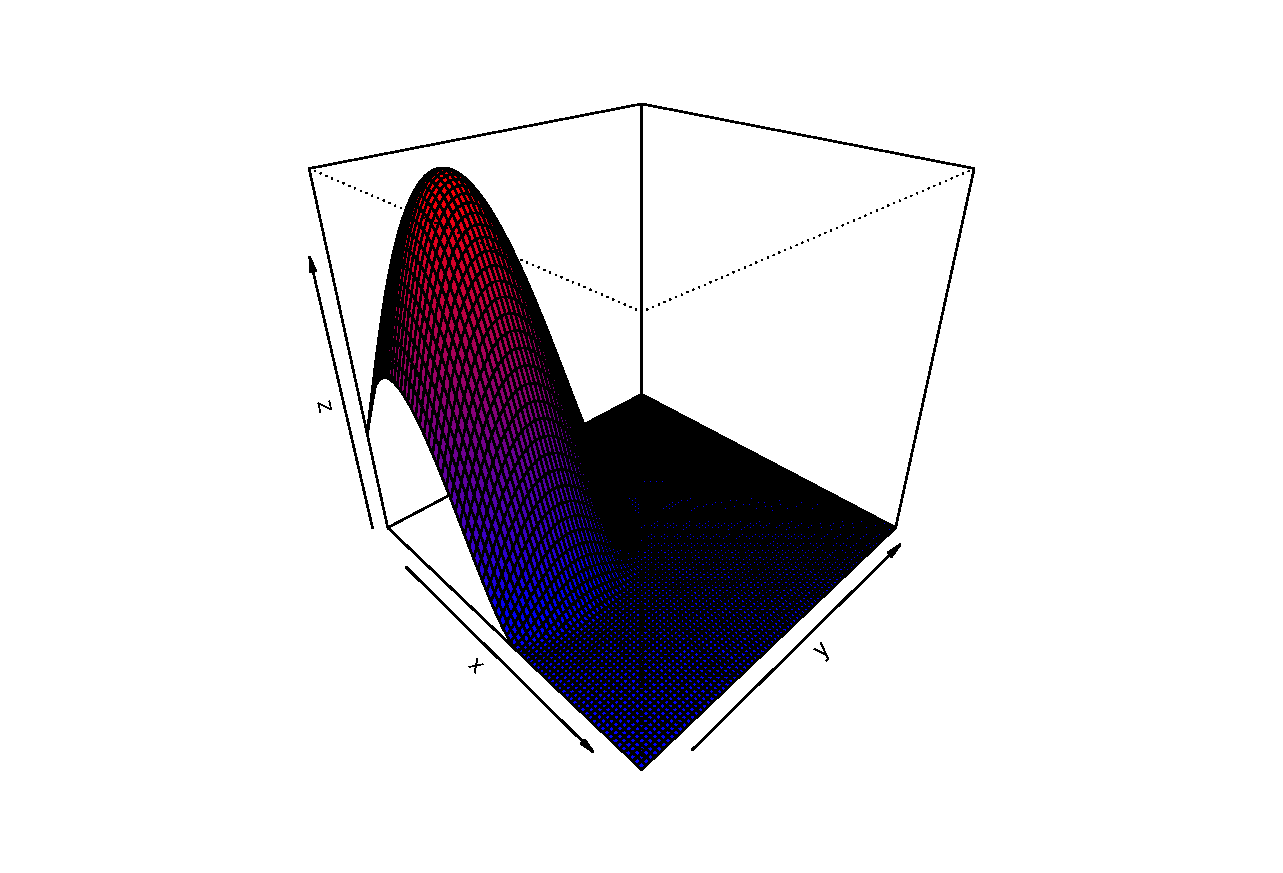
\includegraphics[width=0.55\columnwidth]{./Images/res1}
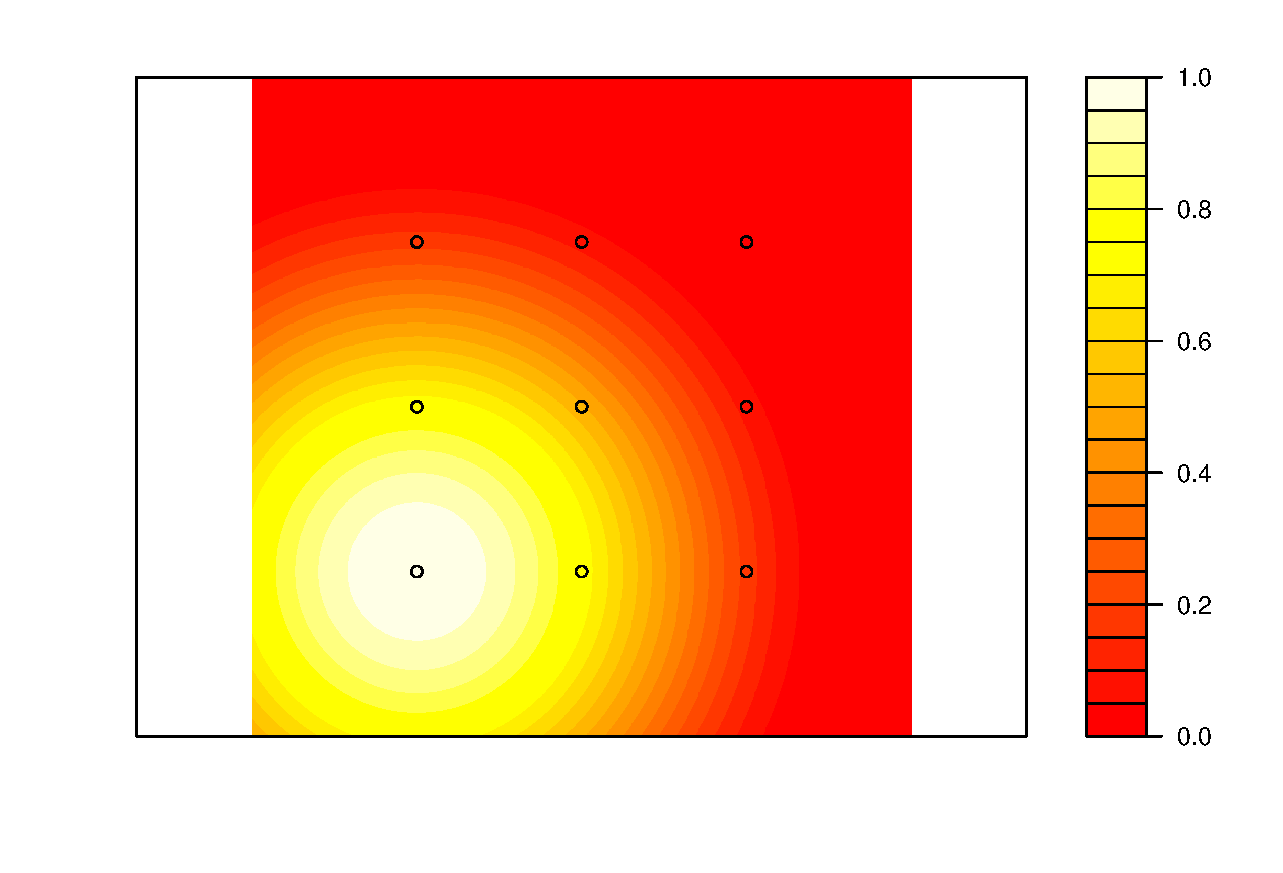
\includegraphics[width=0.44\columnwidth]{./Images/res11}
\caption{}
\label{fig:res1}
\end{figure}

\begin{figure}[!ht]
\centering
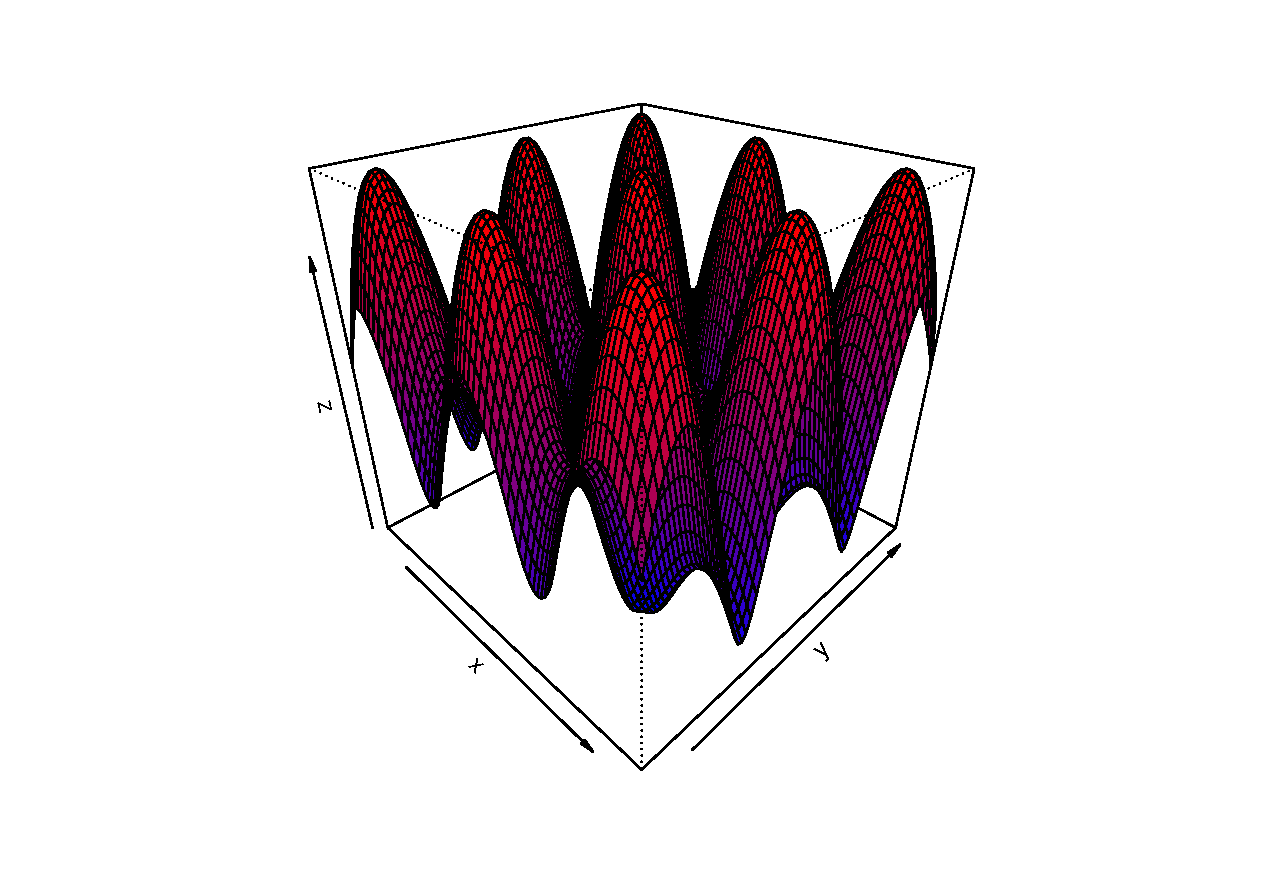
\includegraphics[width=0.55\columnwidth]{./Images/res2}
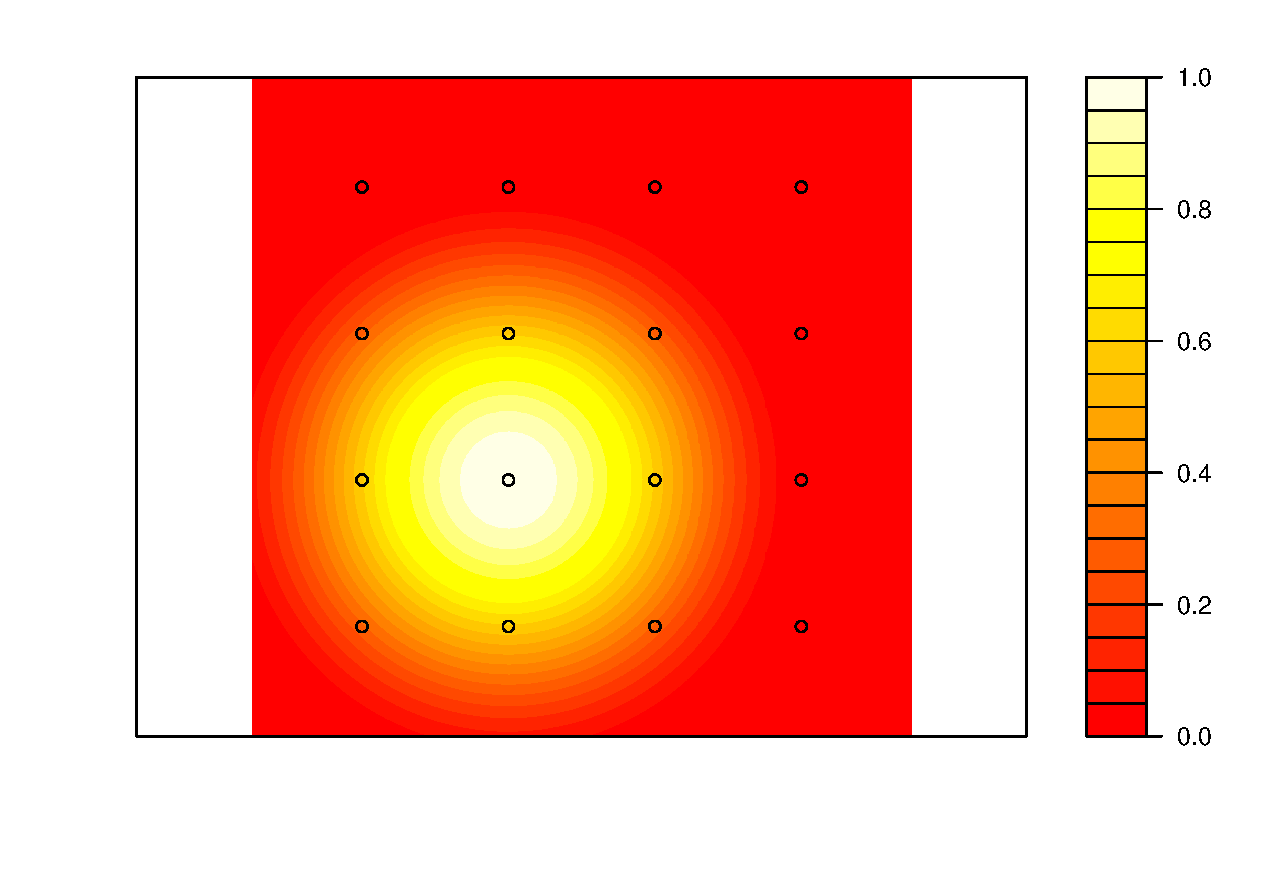
\includegraphics[width=0.44\columnwidth]{./Images/res21}
\caption{}
\label{fig:res2}
\end{figure}

\begin{figure}[!ht]
\centering
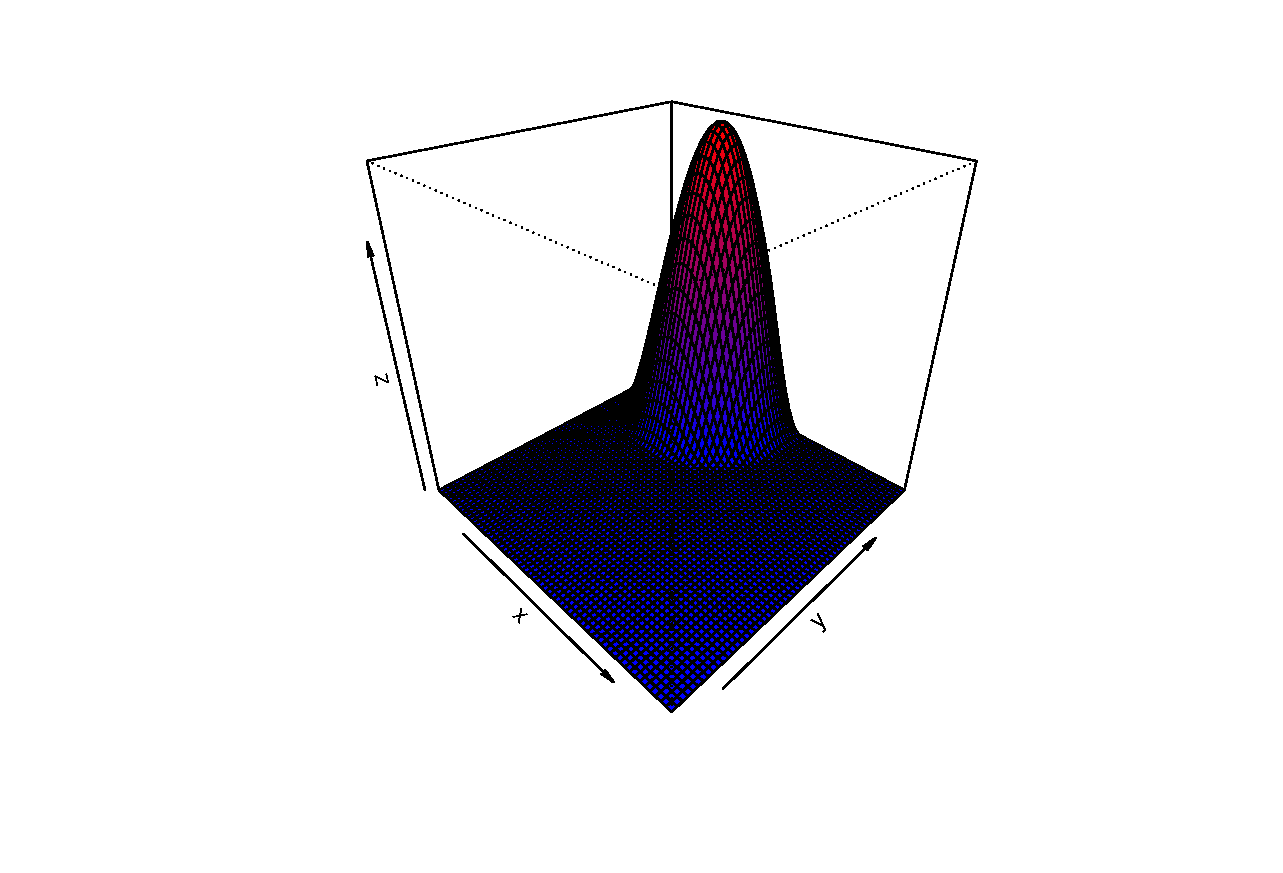
\includegraphics[width=0.55\columnwidth]{./Images/res3}
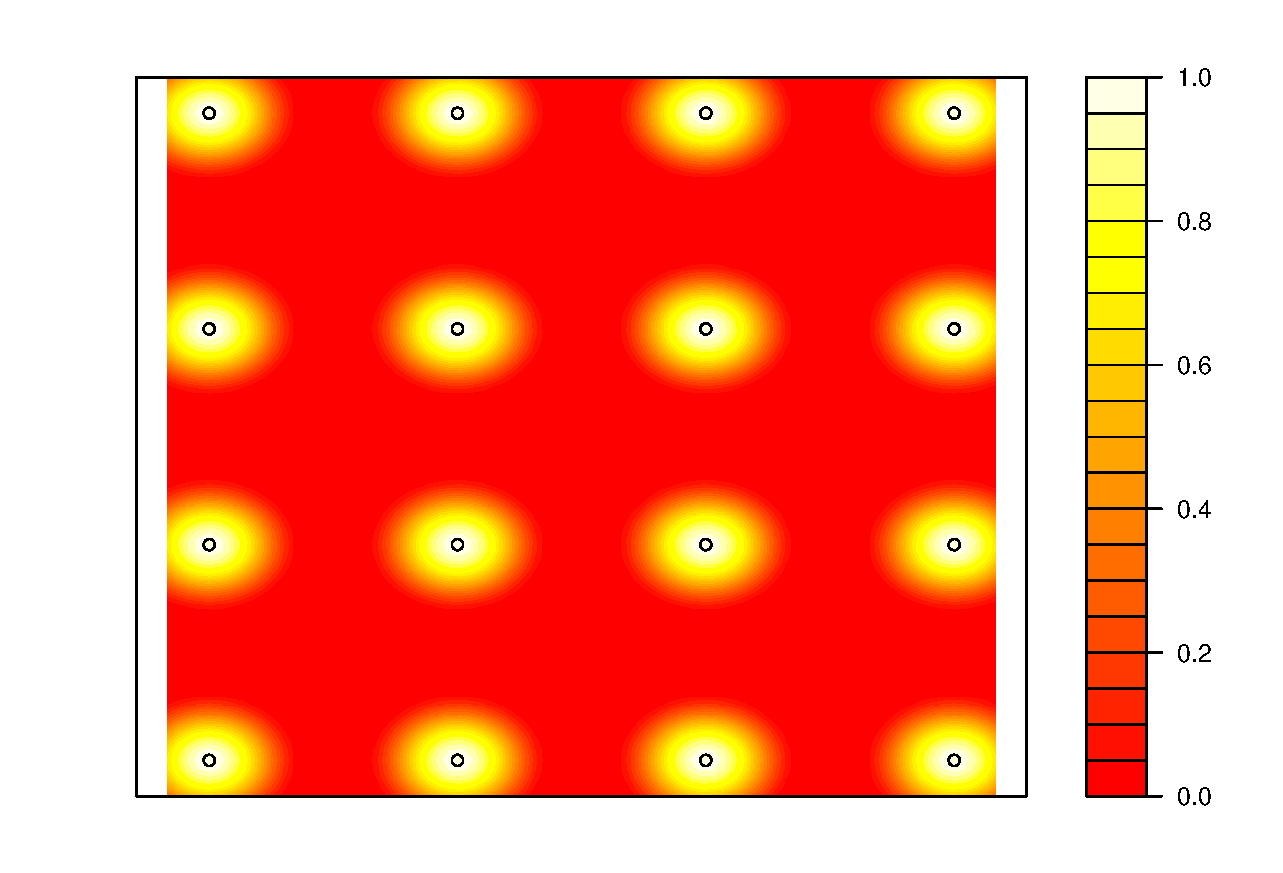
\includegraphics[width=0.44\columnwidth]{./Images/res31}
\caption{}
\label{fig:res3}
\end{figure}

\subsection{Estimation of $\sigma^2_{\epsilon}$ via Semivariogram}

Stuff.\\

\subsection{Estimation of $\sigma^2_{\psi}$ and $K$ via EM Algorithm}

Stuff.\\

\subsection{Fixed Rank Kriging: Smoothing and Prediction}

Stuff.\\


%%%%%%%%%%%%%%%%%%%%%%%%%%%%%%%%%%%%%%%%%%%%%%%%%%%%%%%%%%%%%%%%%%%%
%%                     RESULTS                                    %%
%%%%%%%%%%%%%%%%%%%%%%%%%%%%%%%%%%%%%%%%%%%%%%%%%%%%%%%%%%%%%%%%%%%%
\newpage
\section{3. Results}

Results go here. \\

%%%%%%%%%%%%%%%%%%%%%%%%%%%%%%%%%%%%%%%%%%%%%%%%%%%%%%%%%%%%%%%%%%%%
%%                     DISCUSSION                                 %%
%%%%%%%%%%%%%%%%%%%%%%%%%%%%%%%%%%%%%%%%%%%%%%%%%%%%%%%%%%%%%%%%%%%%
\newpage
\section{4. Discussion}

Discussion goes here. \\

%%%%%%%%%%%%%%%%%%%%%%%%%%%%%%%%%%%%%%%%%%%%%%%%%%%%%%%%%%%%%%%%%%%%
%%                     R APPENDIX & DOCUMENTATION                 %%
%%%%%%%%%%%%%%%%%%%%%%%%%%%%%%%%%%%%%%%%%%%%%%%%%%%%%%%%%%%%%%%%%%%%
\newpage
\section{5. R Code Appendix}

\subsection{Documentation Source}
All project documentation and source code is available in the following github repository. \\

\myindent \underline{https://github.com/jstarling1/spatialsmoothing}

\subsection{R Code: Main Launcher File}


\subsection{R Code: Main Launcher File}


% 
% \subsection{R Code: Main Analysis Code}
% \linespread{1} % Line spacing for R code section.
% \lstinputlisting[language=R,breaklines=true]{"/Users/jennstarling/UTAustin/2016_Fall_SDS 383C_Statistical Modeling 1/Final Project/penalized-matrix-decomp/R Code/383C_FinalProject_RCode.R"}
% 
% \subsection{R Code: Penalized Matrix Decomposition Functions}
% 
% %% Display R script.
% \lstinputlisting[language=R,breaklines=true]{"/Users/jennstarling/UTAustin/2016_Fall_SDS 383C_Statistical Modeling 1/Final Project/penalized-matrix-decomp/R Code/Penalized_Matrix_Decomp_Functions.R"}

\end{document}